\documentclass[conference]{IEEEtran}
\IEEEoverridecommandlockouts
% The preceding line is only needed to identify funding in the first footnote. If that is unneeded, please comment it out.
\usepackage{cite}
\usepackage{amsmath,amssymb,amsfonts}
\usepackage{algorithmic}
\usepackage{graphicx}
\usepackage{textcomp}
\usepackage{xcolor}
\def\BibTeX{{\rm B\kern-.05em{\sc i\kern-.025em b}\kern-.08em
    T\kern-.1667em\lower.7ex\hbox{E}\kern-.125emX}}


\newtheorem{constraint}{\textit{Constraint}}

\newenvironment{defn}
{\vspace{12pt} \noindent {\textit{meaning:}}} \\

\begin{document}

\title{Paper Title*\\
{\footnotesize \textsuperscript{*}Note: Sub-titles are not captured in Xplore and
should not be used}
\thanks{Identify applicable funding agency here. If none, delete this.}
}

\author{\IEEEauthorblockN{1\textsuperscript{st} Given Name Surname}
\IEEEauthorblockA{\textit{dept. name of organization (of Aff.)} \\
\textit{name of organization (of Aff.)}\\
City, Country \\
email address}
\and
\IEEEauthorblockN{2\textsuperscript{nd} Given Name Surname}
\IEEEauthorblockA{\textit{dept. name of organization (of Aff.)} \\
\textit{name of organization (of Aff.)}\\
City, Country \\
email address}
}

\maketitle

\begin{abstract}

\end{abstract}

\begin{IEEEkeywords}
component, formatting, style, styling, insert
\end{IEEEkeywords}

\section{Introduction}
\textbf{par 1} \\
\textit{what is floorplanning and how is it applied (what's its role) in the context of PR, what is the benefit of having a good floorplan or a floorplan at all} \\

\textbf{par 2} \\
\textit{How is fp done currently and what are the shortcomings of those methods} \\

\textbf{par 3} \\
\textit{In short what did I do and what are my contributions (clearly stated)} \\

\textbf{par 4} \\
\textit{organization of the paper} \\

Floorplanning is one of the major challenges in the field of dynamic parital reconfiguration. The placement of the static and reconfigurable slots on the FPGA fabric must satisfy the application requirements set by the application designer while also respecting the technological constraints set by the manufacturer. The conventional approach for an automated generation of FPGA floorplans usually involves two steps. First for each slot, all the possible rectangular slots that satisfy the resources requirement of the slot are enumerated. This is done by starting a scan on the fpga fabric from the bottom left corner and lisitng all the rectangles that contain all the necessary resources for the respective slots. Then some sort of heuristics/optimization is applied to choose the optimal ones from the set of possible slots. This approach has many problems \{\textit{to be listed later}\}\\\\

Our approach instead focuses on applying the optimization process on a lower level of abstraction of the fpga fabric i.e., rather than applying optimization to select the most optimal one from a set of pre-scanned slots, we modeled the different types of resources on the fpga and their distribution along with forbidden regions as a set of constraints and added these constraints to the predefined constraints related to dpr. \\

Let us consider a floorplanning example where we have to make a floorplan for two slots S$_1$ and S$_2$ on the FPGA fabric. Each slot has resource requirements denoted as \{D$_1$, B$_1$, C$_1$\} and \{D$_2$, B$_2$, C$_2$\} where D, B and C represent DSP, BRAM and CLB respectively. \\ Our proposed system takes as an input in the resource requirement of each slot and a description of the resource distribution of the FPGA fabric and it returns the placement coordinates of the slots on the fpga fabric. \\
A slot is represented using 4 parameters i.e. the two bottom left coordinates and the width and the height of the slot. In our considered example the slots S$_1$ and S$_2$ are represented as (x$_1$, y$_1$, w$_1$, h$_1$) and (x$_2$, y$_2$, w$_2$, h$_2$). A forbidden region is also represented as a slot hence a forbidden region F$_i$ can be represented as {fx$_i$, fy$_k$, fw$_i$, fy$_i$}  \\ 



\section{Related Works}
\section{PR floorplanning Problem Description and Considerations}
In this section we breifly describe the general architecture of FPGAs, the design flow in partial reconfiguration (PR) and the assumptions we set to model the PR floorplanning problem as a MILP problem.\\

\subsection{FPGA architecture and Partial-Reconfiguration}
\textbf{\\provide a relevant background on FPGAs, describe the basics of FPGA, how resources are organized,
 talk about tiles of different resources, clock regions, static logic elements etc... 
 Describe everything seen on the picture below} \\
 
\begin{itemize}
\item How is an fpga organized
\item what are clock regions
\item how does PR take place on the circuitry level
\end{itemize}

The reconfigurable fabric of Xilinx FPGAs is divided into quadrants named clock regions. Within each clock region there are grids (columns) of different resources with non uniform distribution. These resource can be CLBs, BRAMs or DSPs.  Resources within a clock region share the same clock. A single column of a specific type of resource in a clock region is referred to as a tile. The number of resources in a tile varies depending on the device family. For example in Virtex 7z a CLB tile contains 50 clbs a BRAM tile contains 10 brams and a DSP tile contains 20 dsps. In addition to the above mentioned resources, FPGAs also contain other components related to clock and clock modifying logic, I/O logic, configuration and debug logic etc..., Depending on the type of device family these components may or may not be included in a reconfigurable region. \\

The configuration memory, which stores the bit file that contains configuration information for both the logic and routing resources on the FPGA, is  organized into minimal configurable units called frames. A single frame in the configuration memory is mapped into a single tile on the fabric. \\

\textbf{put picture detailing FPGA architecture} \\

Reconfigurable regions are rectangular in shape and to ease the routing and placement during implementation, the height of the reconfigurable region must be aligned to clock region boundareis. \\

Partially reconfigurable applications are often composed of static and reconfigurable modules which respectively reside in the static and reconfigurable regions on the FPGA fabric. Partial-reconfiguration fundamentally involves dynamically switching modules in a reconfigurable region whilst other reconfigurable and static regions continue to be operational. As tiles are the minimal configuration unit in an FPGA, two reconfigurable regions must not share a tile. \\ 
 
\subsection{Consideration for resource representation}
\textbf{\\state how the fpga is divided into x-y coordinate system. Explain how current genaration of xilinx fpgas differ in resource distribution on the fabric} \\

As shown in the figure, a cartesian coordinate system can be overlayed on FPGAs to identify each resource on the logic fabric. The x axis represents each column of resources while each row on the y axis represents a clock region. Hence resources are organized on a tile basis instead of being individually located as single clb, bram or dsps. This configuration matches the minimal reconfiguration unit philosophy of PR. \\

A reconfigurable region R$_i$ is hence represented with (x$_i$, y$_i$, w$_i$, h$_i$) where x$_i$ and y$_i$ are the bottom left coordinate of R$_i$ and w$_i$ and h$_i$ are the width and height respectively. \\

 
%The total number of a resource R within a slot S$_i$ = (x$_i$, y$_i$, w$_i$, h$_i$) is then equal to
%\begin{equation}
%R = (x_i + w_i) \cdot (y_i + h_i)
%\end{equation}  

\subsection{transformation to binary}
\textbf{\\why do we need to linearize the grids and which grid is better to linearize. Justtify with a practical example.}\\

A reconfigurable region, R$_i$, must contain at least the necessary number of resources required by a module that is going to be placed. Determining the number of resource contained in R$_i$ invloves determining the area of the rectangle. In formulating PR-floorplanning as a linear optimization problem the resource requirement constraints must also be linear. Hence to satisfy the condtion of modeling the resource requirement as a linear constraint either of the axis' must be discretized. Deciding which axis to discritize is an important design decision since reducing the number of binary variables leads to a scalable model. In all the FPGA families that were chosen to be studied for this project, the number of rows (the number of clock regions on the y axis) was less than the number of columns on the x axis. For example in kintex xc7z045fbv676 there are 100 columns on the x axis as opposed to 7 rows on the y axis.\\


\subsection{FPGA resource finger-printing} 
\textbf{\\what is fpga resource finger printing ? Plot a piecewise linear graph of a clb in a single row or put the function description of the piecewise linear graph} \\

\begin{itemize}
\item Joining two adjacent clock regions resources on a single row can be described from 0 to W-1
\item the structure is regualr and it will repeat itself 
\item discontinuties are modeled with forbidden regions
\item Put a picture of the zynq implemenetaion and describe the clbs brams and dsp and plot the piecewise graph
\end{itemize}



The resources on FPGAs are not distributed uniformly which means  distributed. This means have 

The FPGA is now abstracted using binary variables on the y axis and integers on the x axis. The fpga is also divided into clock regions. A clock regions spans r rows high. The total number of rows, which is designated as H, is the sum of rows in all clock regions {0... clk\_reg} i.e.,  
\begin{equation}
H = \sum_{j=0}^{clk\_reg} r
\end{equation}

The distribution of each resource on the x axis of the FPGA in a single row can be represented using a piece-wise linear function. For example in zynq xc7z015 the number of clbs on the x axis between the bottom left corner i.e., (0, 0) and a point x, on the x axis is represented using F(x) as  

\begin{equation}
F(x) = \begin{cases}
x, & \textbf{ 0$\leq$x$<$4}, \\
(x-1), & \textbf{4$\leq$x$<$7}, \\
(x-2), & \textbf{7$\leq$x$<$10}, \\
(x-3), & \textbf{10$\leq$x$<$15}, \\
(x-4), & \textbf{15$\leq$x$<$18}, \\
(x-5), & \textbf{18$\leq$x$<$22}, \\
(x-6), & \textbf{22$\leq$x$<$25}, \\
(x-7), & \textbf{25$\leq$x$<$W},
\end{cases}
\end{equation}

The number of clb, in a height of a single row, between x$_i$ and x$_k$ where x$_i$ $\geq$ x$_k$ can then be represented as clb(x$_i$, x$_k$) such that 

\begin{equation}
clb(x_i, x_k) = F(x_k) - F(x_i)
\end{equation}

if $\beta_{ijk}$ represents row k in clock region j for slot i on the fpga then C(x$_i$, y$_i$, w$_i$, h$_i$) which is the total number of clbs in a slot S$_i$ can be calculated as 
\begin{equation}
C(x_i,y_i,w_i,h_i) = \sum_{j=0}^{clk\_reg} \sum_{k=0}^{r-1} \beta_{ijk} \cdot (F(x_i+w_i) - F(x_i))
\label{clb_tot}
\end{equation}
where h$_i$ which is the height of S$_i$ and can be expressed as 

\begin{equation}
h_i = \sum_{j=0} ^{clk_reg} \sum_{k=0}^{r-1} \beta_{ijk}
\end{equation}

The same resource finger-printing using piecewise linear functions can be done to the bram and dsp on the fpga and this can then be used to determine the amount of a specific type of resource within a slot.

\section{Background and Modeling}
In this section we breifly describe the general architecture of FPGAs, the design flow in partial reconfiguration (PR) and the assumptions that led to the fromulation of PR floorplanning problem as a MILP problem. This work is based on the 7 series FPGA family from Xilinx. \\

\subsection{FPGA Architecture and Partial-Reconfiguration}

The configurable fabric of Xilinx FPGAs is divided into quadrants named clock regions. Within each clock region there are columns of different configurable resources such as CLBs, BRAMs or DSPs.  Resources within a clock region share the same clock. A single column in a clock region is referred to as a tile. The number of resources in a tile varies depending on the device family. For example in Virtex 7z a CLB tile contains 50 clbs a BRAM tile contains 10 brams and a DSP tile contains 20 dsps. The functional logic compoenets (clbs, brams and dsps) and the routing logic components (switches, interconnects etc...) on the FPGA are configured based on a bit file stored in the configuration memory of an FPGA. This memory is organized into minimal configurable units called frames. A single frame in the configuration memory corresponds to a single tile on the fabric. In addition to the above mentioned resources, FPGAs also contain other components such as clock and clock modifying logic, I/O logic, configuration logic etc... Depending on the type of device family some of these components may or may not be included in a reconfigurable region. FPGAs, in particular 7 series devices, which are subject of this work, also contian routing resources called interconnect tiles. These tiles are placed back-to-back as shown in Fig \ref{fig:fpga}. When floorplanning for partial reconfiguration, the position of these back-to-back boundaries must be known inorder not to split them and violate PR restriction.

\begin{figure}
  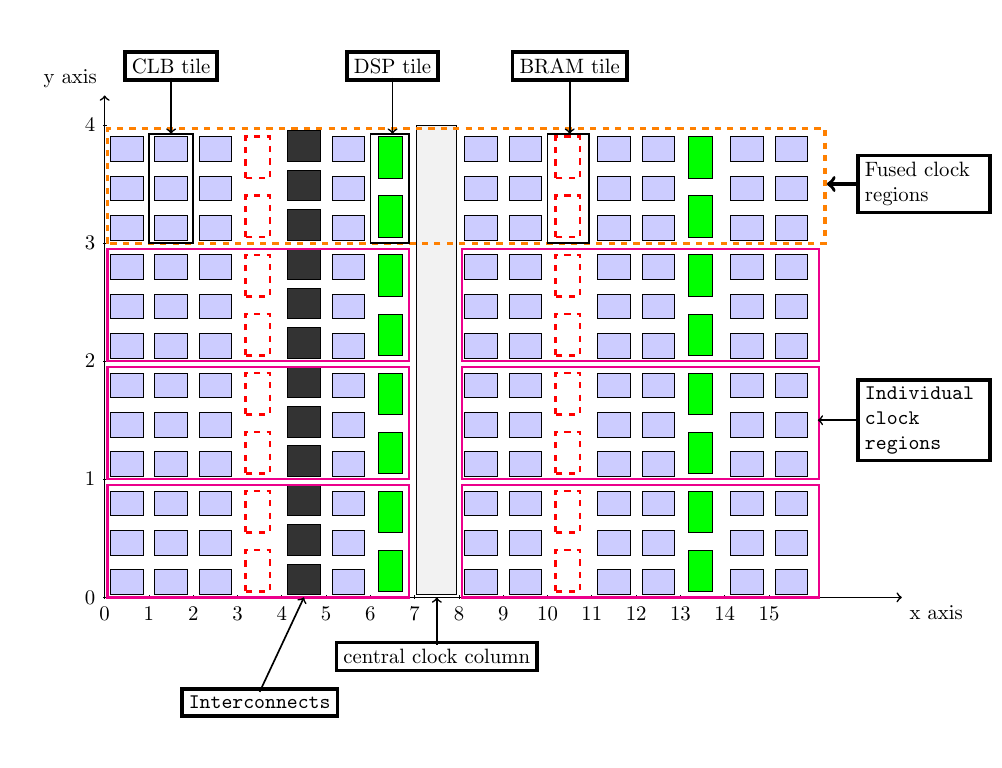
\includegraphics[width=\linewidth]{graphics/fpga.png}
  \caption{FPGA architecture}
  \label{fig:fpga}
\end{figure}

Partially reconfigurable applications are often composed of \textbf{\textit{M$_s$}} number of static and \textbf{\textit{M$_r$}} number of reconfigurable modules that are to be placed in \textbf{N$_s$} static and \textbf{N$_r$} reconfigurable regions on the FPGA respectively.  In PR applications the number of static modules equals to the number of static regions i.e., \textit{M$_s$ = N$_s$} while the number of reconfigurable modules is always greater than reconfigurable regions i.e., \textit{M$_r$ $>$ N$_r$}. Floorplanning in PR can then be defined as the process of allocating placement for \textit{N$_r$} reconfigurable regions on the FPGA fabric. \\

\textbf{state how PR-fp is currently done in vivado} \\

\subsection{Combining clock regions}
On Xilinx FPGAs, the central clock column divides the FPGA into left and right regions as shown on fig \ref{fig:fpga}. But in our model all the horizontally adjacent clock regions were fused into a single clock region. This simplifies our modeling with no penalty. As also shown in the figure on fig \ref{fig:fpga}, a cartesian coordinate system can be overlayed on FPGAs to uniquely identify each resource on the logic fabric. The x axis represents each column of resources while the rows on the y axis represent the fused horizontally adjacent clock regions as indicated on fig \ref{fig:fpga}. Combining the horizontally adjacent clock regions\footnote{henceforth clock regions implies horizontally fused clock regions}, in addition to resulting in a lower range of variables on the y axis, organizes resources on the y axis on a per tile (per clock region) basis instead of as individual clbs, brams or dsps. This reduces the search space for the solution in the MILP formulation at the expense of wasting resources. Based on this abstraction the resources on the FPGA fabric on a tile basis, the FPGA would become \textbf{W} columns wide and \textbf{H} clock regions high.  \\

The i\textsuperscript{th} reconfigurable region R$_i$ is a rectangular region on the FPGA fabric that hosts, at different durations, the set of reconfigurable modules assigned to it. R$_i$ can be represented as
\begin{equation}
R_i = (x_i, y_i, w_i, h_i) \mid x_i + w_i \leq W, y_i + h_i \leq H
\end{equation}

where x$_i$ and y$_i$ represent the bottom left coordinate and w$_i$ and h$_i$ represent the width and height of R$_i$ resectively. A resource type \textit{t} that is required by reconfigurable module \textit{M$_r$} is denoted as \textit{c$_{rt}$} while the same type of resource that is incorporated inside a reconfigurable region R$_i$ is denoted as $\eta_{it}$. The upper and lower boundaries of R$_i$ are aligned to clock region boundaries since the resources on the fabric are organized on a tile basis. 

\textbf{\\talk about the modeling of forbidden regions}

\subsection{Discretization of the axis}
Floorplanning is a two dimensional (quadratic) problem in that determining the number of resource contained in R$_i$ invloves determining the resources on both axis i.e., the area of the rectangle. To linearize this problem either of the axis must be discretized. A good strategy for discretization would be choosing the axis with the lower range of variables as this leads to an easily scalable model. In all the FPGA families that were chosen to be studied for this project, the range of the y axis (the number of clock regions on the y axis) was less than the range of the x axis i.e., H $<$ W. For example in kintex xc7z045fbv676 there are 100 columns on the x axis as opposed to 7 clock regions on the y axis. Hence the binary variable $\beta_{ij}$ denotes clock region j in region in R$_i$. \\

%$\forall$ i = 1...,N$_r$,  $\forall$ j = 1...,H \\
%$\beta_{ij}$ $\in$ [0,1] $\mid$ $\beta_{ij}$ represents clock region j in R$_i$. \\

\subsection{FPGA resource finger-printing} 
Resources in most Xilinx FPGAs are distributed in a redundant manner this is to say vertically adjacent clock regions have a fairly similar distribution of resources with the possibility of different forbidden regions being included in them. Hence the reconfigurable fabric of most Xilinx FPGAs can accurately be represented by describing the resources in a single clock region and the location of forbidden regions in all clock regions. This process is equivalent to developing the resource distribution finger-print of a specifc type of FPGA. For each resource type \textit{t} a piecewise function f$_t$(x) can be used to describe the distribution of that particular resource inside the first clock region of the FPGA along the x axis. As an example f$_t$(x) for the first clock region on fig \ref{fig:fpga} would be 

\begin{figure}
  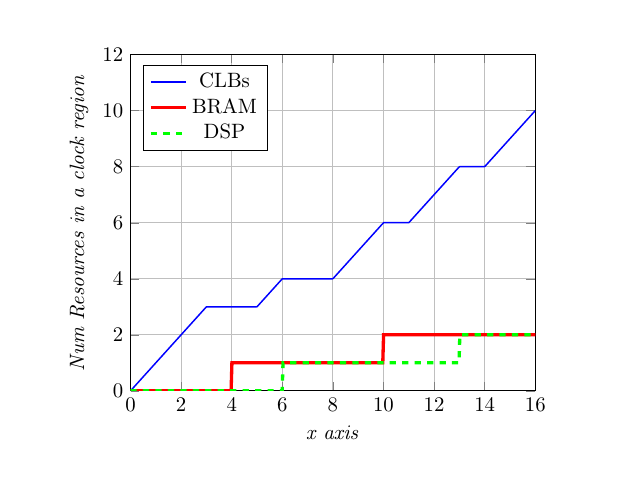
\includegraphics[width=\linewidth]{graphics/resource.png}
  \caption{Resource distribution finger print of fig \ref{fig:fpga}}
  \label{fig:finger-print}
\end{figure}


\begin{comment}
\begin{equation}
f_c(x) = \begin{cases}
\mu_c * x, & \textbf{ 0$\leq$x$<$4}, \\
\mu_c * (x-1), & \textbf{4$\leq$x$<$7}, \\
\mu_c * (x-2), & \textbf{7$\leq$x$<$W}, \\
\end{cases}
\end{equation}
\end{comment}

%\textbf{fig} depicts f$_t$(x) for the first clock region zynq xc7z015.

If $\mu_t$ is a constant that denotes the number of resource \textit{t} per tile, the amount of each type of resource included inside a region R$_i$ i.e., $\eta_it$ can be defined as \\

\begin{equation}
\label{model:eq:4}
\eta_{it} = \sum_{j=1}^{H} \beta_{ij} \cdot (f_t(x_i+w_i) - f_t(x_i)) * \mu_t
\end{equation}

\begin{comment}
The set of components that must not be included in 
A reconfigurable region R$_i$ must, at the very least, incorporate the resources required by the largest reconfigurable module that it hosts. Reconfigurable regions are rectangular in shape and to ease the routing during implementation, the height of the reconfigurable region must be aligned to clock region boundaries.\\
\end{comment}

\section{Experiemtnal Results}
\subsection{Experimental Setup}
How was the experiment implmented i.e, with what kind of prog. langaguge, on what optimization tool, on what platforms...
What is the system being tested for ? What is the compositon of the synthethic task suite used for testing. What type of FPGAs are modeled ?  What are the challenges when switiching between models.  \\


The system is tested for Exec time Vs Num of Reconfigurable regions and Exec time Vs \%of resources used by the system on both zynq and virtex\\

The system is also tested for \% of wasted resources (coeficients used to set allowed percentage of resources to be wasted \%)VS Exec time on both virtex and zynq. The average wasted resources are also reported when not imposing these constraints and what effect it has on exec time and feasibility in general. my guess is that upto a certain point (upto a certain \% of utilization of resources) not imposing these constraints improves the exec time but after the utilization increases (i.e., more applications require more resources) not imposing these coeffecients leads to infeasible constrants. This has to be tested with a carefully designed test suit which will test the limist of the platform. \\

Finally a case study on a real application on Zynq. 


\end{document}
